Clase: 25/08/2022

\begin{prop}
    Sea $f$ una función definida y analítica sobre una región (Dominio: abierto y conexo)$G\subset \mathbb{C}$, y si $f'(z)=0,\forall z\in G$, entonces $f$ es constante.
    \begin{dem}
        Sea $z_0\in G$ un punto en $G$ (fijo) y sea cualquier $z\in G\implies$ por el T.F.C.
            $$\int_\gamma f'(z)dz=f(z)-f(z_0),$$
            donde $\gamma$ es una curva que une $z_0$ con $z$. $\implies$ como $f'(z)=0,\forall z\in\mathbb{C}\implies \int_\gamma f'(z)dx=0\implies f(z)=f(z_0),\forall z\in G\implies f$ es constante. 
    \end{dem} 
\end{prop}

\begin{ejemplo}
    \begin{enumerate}
        \item Sean $z_1=1,z_0=-1$ y $f(z)=3z^2$. $\implies \int_\gamma f(z)dz=\int_\gamma 3z^2dz=z^3|_{z_0}^z=1^3-(-1)^3=2$. Para cualquier curva $\gamma$.
        \item Sea $z_1=-1,z_0=1$ y $f(z)=1/z$.
        \begin{enumerate}
            \item Considere $\gamma$: el semicirculo unitario superior.Sea $\gamma(t)=e^{it}=\cos t+i\sin t,\quad 0\leq t\leq \pi$
            $$\int_\gamma \frac{1}{z}dz=\int_0^\pi \frac{1}{e^{it}}\cdot ie^{it}dt = \pi i$$
            \item Considere $\gamma$: el semicirculo unitario inferior.Sea $\gamma(t)=e^{-it},\quad 0\leq t\leq \pi$
            $$\int_\gamma \frac{1}{z}dz=\int_0^\pi \frac{1}{e^{-it}}\cdot (-i)e^{-it}dt = -\pi i$$
        \end{enumerate}
        
    \end{enumerate}
\end{ejemplo}

\begin{teorema}[Independencia de trayectorias]
    Suponga que $f$ es una función continua sobre una región $G\subseteq \mathbb{C}$. Los enunciados siguientes son equivalentes:
    \begin{enumerate}
        \item Las integrales son independientes de la curva: si $z_0,z_1\in G$ y si $\gamma_1,\gamma_2$ son curvas de $z_0$ a $z_1$ sobre $G$, entonces:
            $$\int_{\gamma_1}f=\int_{\gamma_2}f$$
        \item Las integrales sobre las curvas cerradas son cero. Si $\gamma$ es curva cerrada en $G$, entonces 
        $$\int_\gamma f=0$$
        \item Existe una antiderivada para $f$ sobre $G$. Existe una función $F$ definida y analítica sobre $G\ni$
        $$F'(z)=f(z),\forall z\in G$$
    \end{enumerate}
\end{teorema}

\begin{ejemplo}
    \begin{enumerate}
        \item Calcule $\int_\gamma xdz$, donde $\gamma$ es el cuadrado unitario.
        \begin{figure}[H]
            \centering
            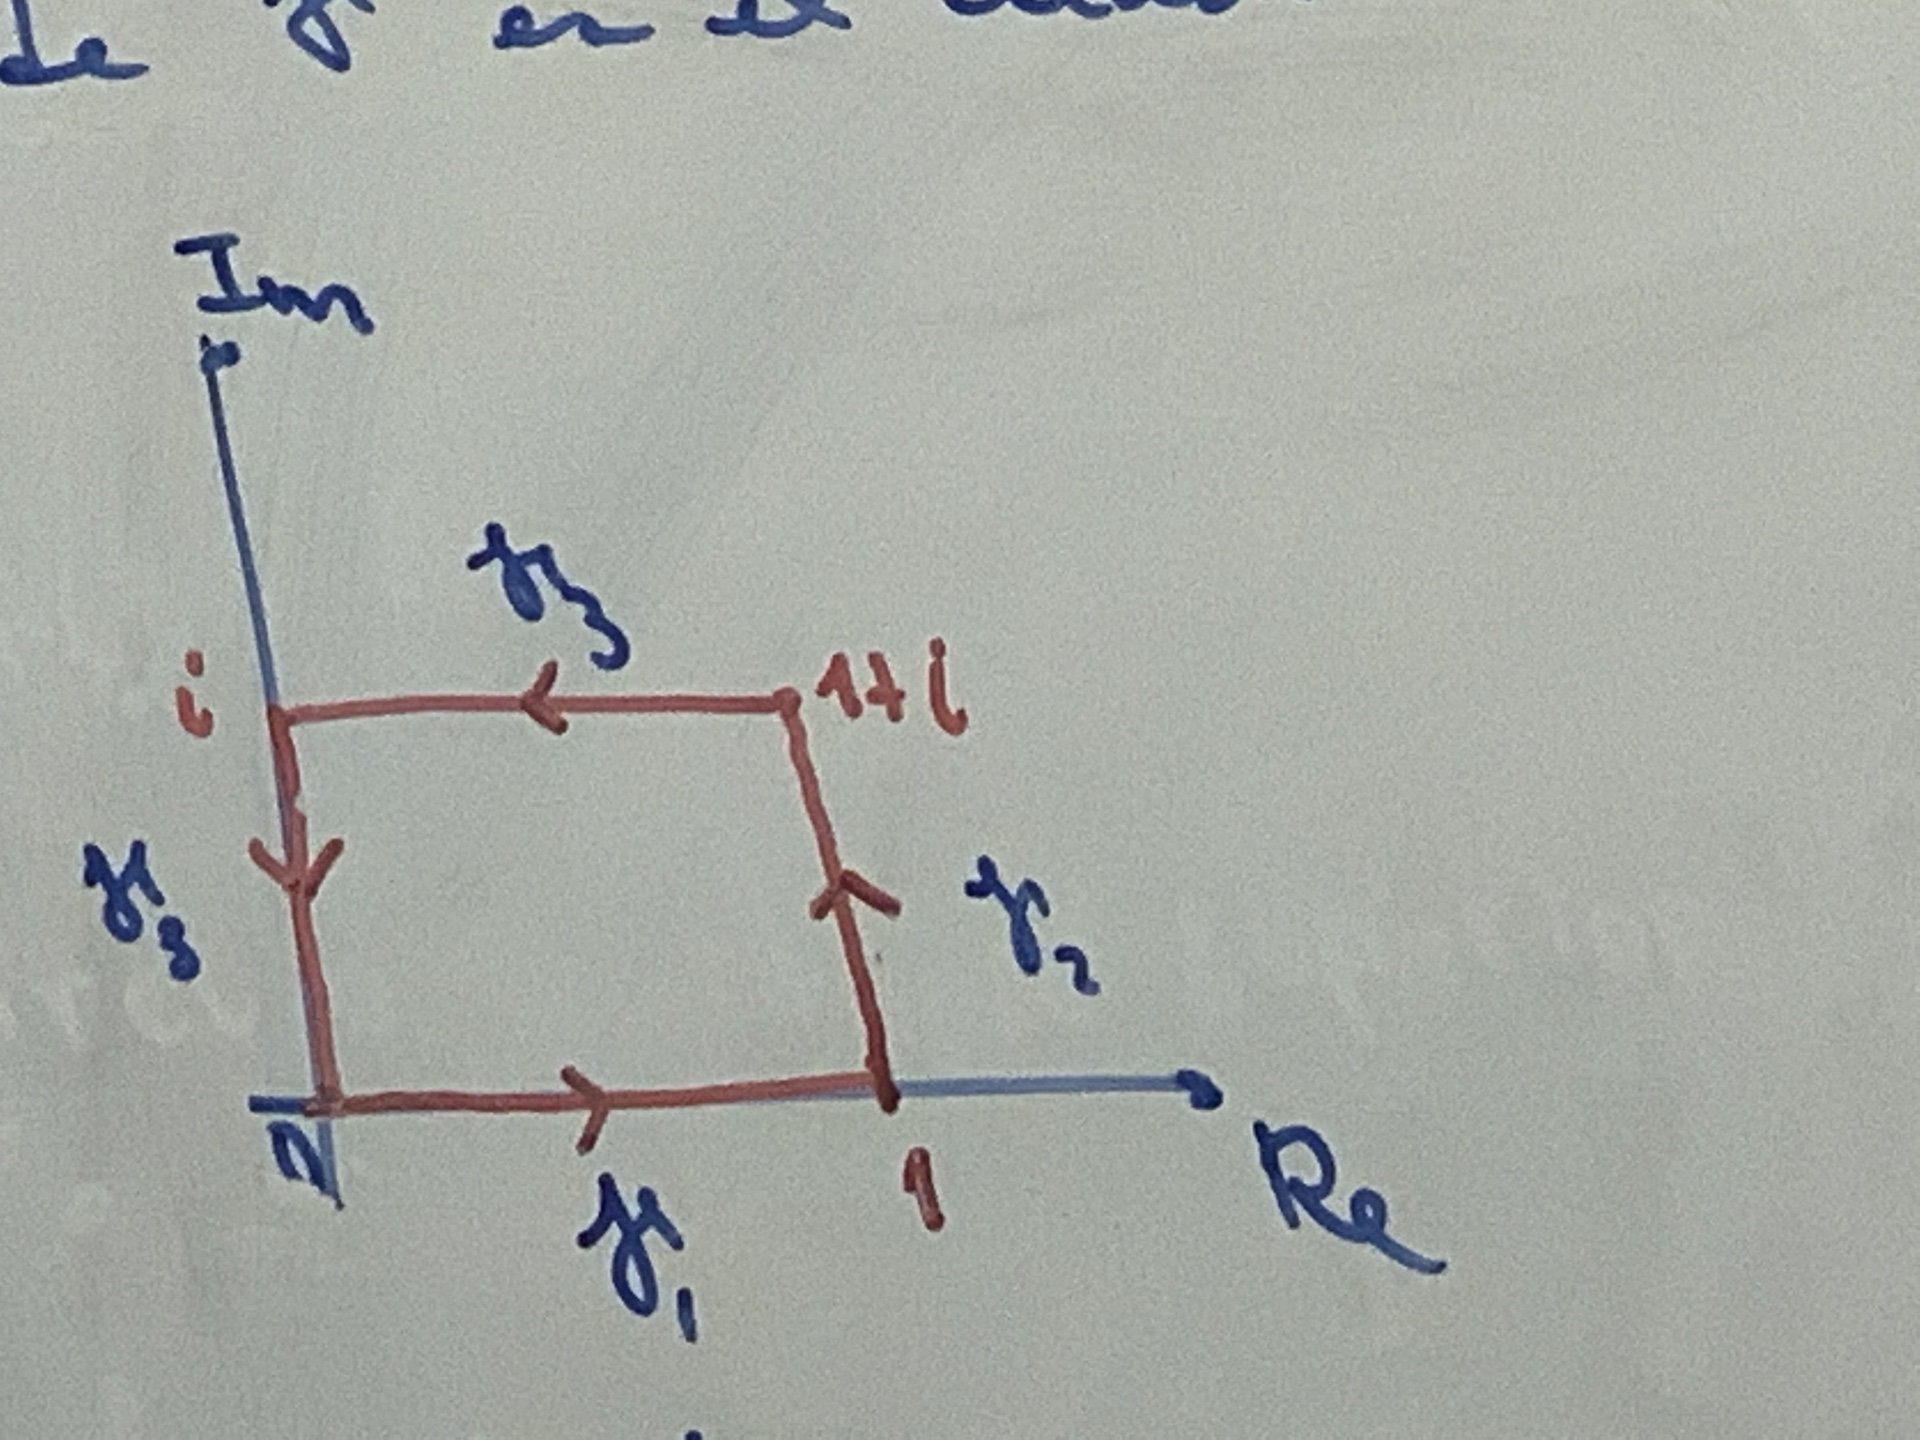
\includegraphics[scale=0.1]{imagenes/8-25-1.jpeg}
        \end{figure}
        \begin{align*}
            \int_\gamma xdz &=\int_\gamma \operatorname{Re}(z)dz\\
            &=\int_{\gamma_1+\gamma_2+\gamma_3+\gamma_4} \operatorname{Re}(z)dz\\
            &=\int_{\gamma_1} \operatorname{Re}(z)dz+\int_{\gamma_2} \operatorname{Re}(z)dz+\int_{\gamma_3} \operatorname{Re}(z)dz+\int_{\gamma_4} \operatorname{Re}(z)dz\\
        \end{align*} 
        Un caso de parametrización: 
        \begin{align*}
            \gamma_1:[0,1]\to \mathbb{C}\ni \gamma_1(t) &= t+0i\\
            \gamma_2:[1,2]\to \mathbb{C}\ni \gamma_2(t) &= 1+i(t-1)\\
            \gamma_3:[2,3]\to \mathbb{C}\ni \gamma_3(t) &= (3-t)+i\\
            \gamma_1:[3,4]\to \mathbb{C}\ni \gamma_4(t) &= 0+(4-t)i
        \end{align*}
        Tenemos las integrales:
        \begin{align*}
            \int_{\gamma_1}f &=\int_0^1 z\cdot 1 dt = \frac{1}{2}\\
            \int_{\gamma_2}f &= \int_1^2 1\cdot i dt = i\\
            \int_{\gamma_3}f &= \int_2^3 (3-t)(-1)dt = -\frac{1}{2}\\
            \int_{\gamma_4}f &=\int_3^4 0dt=0
        \end{align*}
        Entonces la suma es $i$. 
    \end{enumerate}
\end{ejemplo}

\begin{ejemplo}
    Calcule $\int_\gamma e^z dz$, donde $\gamma$ es la parte del circulo unitario que une 1 con $i$. 
    \begin{figure}[H]
        \centering
        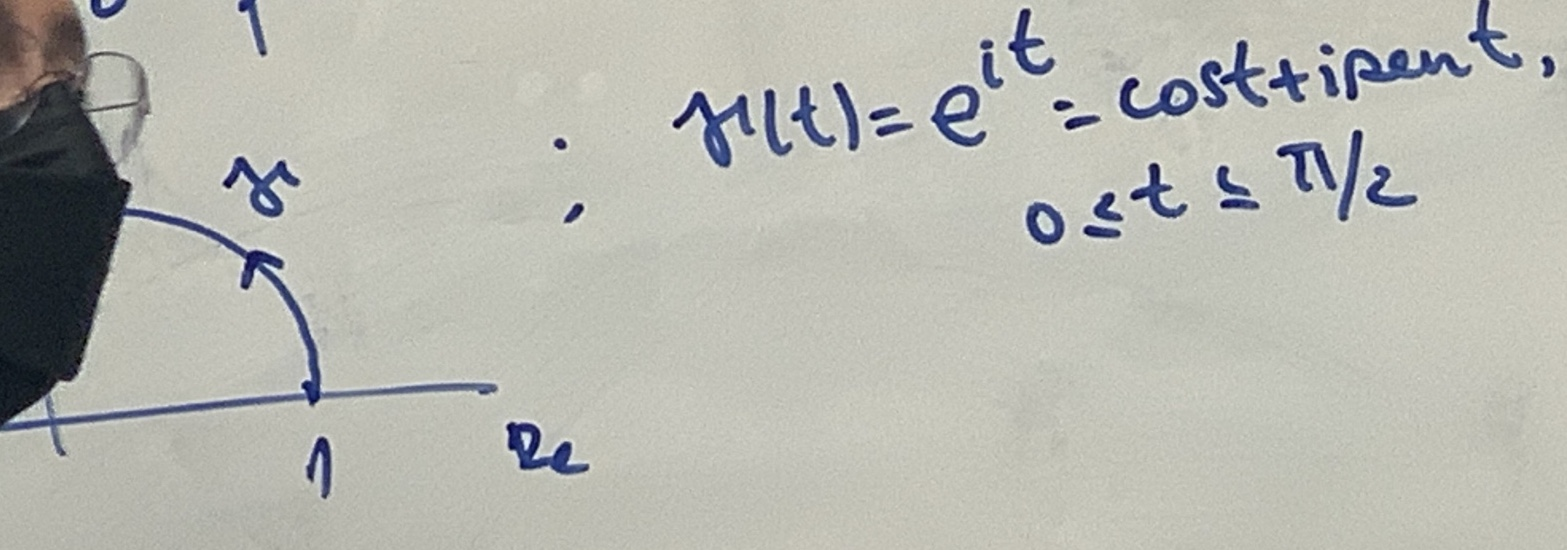
\includegraphics[scale=0.1]{imagenes/8-25-2.jpeg}
    \end{figure}
    \begin{enumerate}
        \item T.F.C $\implies \int_\gamma e^z dz=e^i-e^1$
        \item Por definición 
        $$ \int_\gamma e^z dz =\int_0^{\pi/2}e^{\cos t + i\sin t}[-\sin t + \cos t]dt$$
    \end{enumerate}
\end{ejemplo}

\begin{ejemplo}
    Calcule $\int_\gamma\frac{dz}{z-a}$, donde $\gamma(t)=a+re^{it},0\leq t\leq 2\pi$
    \begin{align*}
        \int_\gamma \frac{dz}{z-a} &= \int_0^{2\pi}\frac{rie^{it}}{a+re^{it}-a}dt\\
        &= \int_0^{2\pi}idt\\
        &= 2\pi i
    \end{align*}
\end{ejemplo}

\begin{ejemplo}
    Encuentre un número $M\ni \left|\int_\gamma \frac{dz}{z^2+2}\right|\leq M$, donde $\gamma$ es el semicirculo unitario superior. 
    \begin{sol}
        Si $|f(z)|=|\frac{1}{z^2+z}|\leq K,K\geq 0$, entonces: 

        $$\left|\int_\gamma \frac{dz}{z^2+z}\right|\leq K\cdot l(\gamma )$$

        Sea 
        $$|z^2+2|=|2+z^2|\geq |2|-|z^2|=2-|z|^2 = 2-1 =1\implies |\frac{1}{z^2+2}|\leq 1$$
        Además, $l(\gamma)=\pi(1)=\pi$. 
        $$\implies \left|\frac{dz}{z^2+2}\right|\leq \pi$$
    \end{sol}

\end{ejemplo}

\begin{teorema}[De Cauchy - Versión intuitiva]
    Suponga que $f$ es analítica sobre y en el interior de una curva cerrada y simple $\gamma$. Entonces, 
    $$\int_\gamma f=0$$
\end{teorema}